\subsubsection*{Analysis}
\begin{tabular}{@{}l l}
\textbf{Scope}:&The AuctionHouse\textsuperscript{TM} automated administration system\\
\textbf{Level}:&User goal\\
\textbf{Primary Actor}:&Owner\\
\textbf{Stakeholders and Interests}:&\begin{tabular}[t]{@{}l}
	Owner: wants to register the search request.\\
	Customer: wants their search request to be registered by the owner.\\
	Search System: wants the new search request to be recorded.\end{tabular}\\
\textbf{Preconditions}:&\begin{tabular}[t]{@{}l}
	User is identified and authenticated.\\
	The customer is registered to the system as a regular customer\\\end{tabular}\\
\textbf{Postconditions}:&\begin{tabular}[t]{@{}l}
	The search request is registered in the system.\end{tabular}\\
\textbf{Special requirements}:&\begin{tabular}[t]{@{}l}-\end{tabular}\\
\textbf{Frequency of occurence}:& \begin{tabular}[t]{@{}l}Varies greatly, from 3 times a day, to once a week.\\Estimated to be 12 times per month.\footnotemark\end{tabular}
\end{tabular}\\\\
\footnotetext{The numbers came from a contact session with John. Session details are in the references, page \pageref{conv1}}
\textsl{Main Success Scenario}
\begin{enumerate}[noitemsep]
	\item The user starts the `file search request' transaction with the system, having all parameters of the user to be added ready.
	\item The system returns a list of all ``Regular Customers'' that have paid the search system registration fee and a list of ``Item Catalogues'' to the user.
	\item The user chooses the customer from the first list and a item catalogue (if so desired; may be ignored) and presents the selections to the system, along with a maximum price the customer is willing to pay.
	\item The system creates the search request with the item catalogue, the maximum price and the customer interested and adds it to the search system's list. The system also generates a Search ID for the request for reference.
	\item The system informs the customer via email that the request has been made.
	\item The system returns to the user with a confirmation message containing the Search ID, or a failure.
\end{enumerate}
\textsl{Extensions}
\begin{itemize}[noitemsep]
	\item 3a. When not all required parameters were provided, the system will first ask the user to provide it until all parameters is provided.
	\item 4a. If the fee has not been paid, the system will return a failure and ends the transaction.
\end{itemize}
\newpage
\textsl{System Sequence Diagram}
\begin{figure}[H]
	\centering
	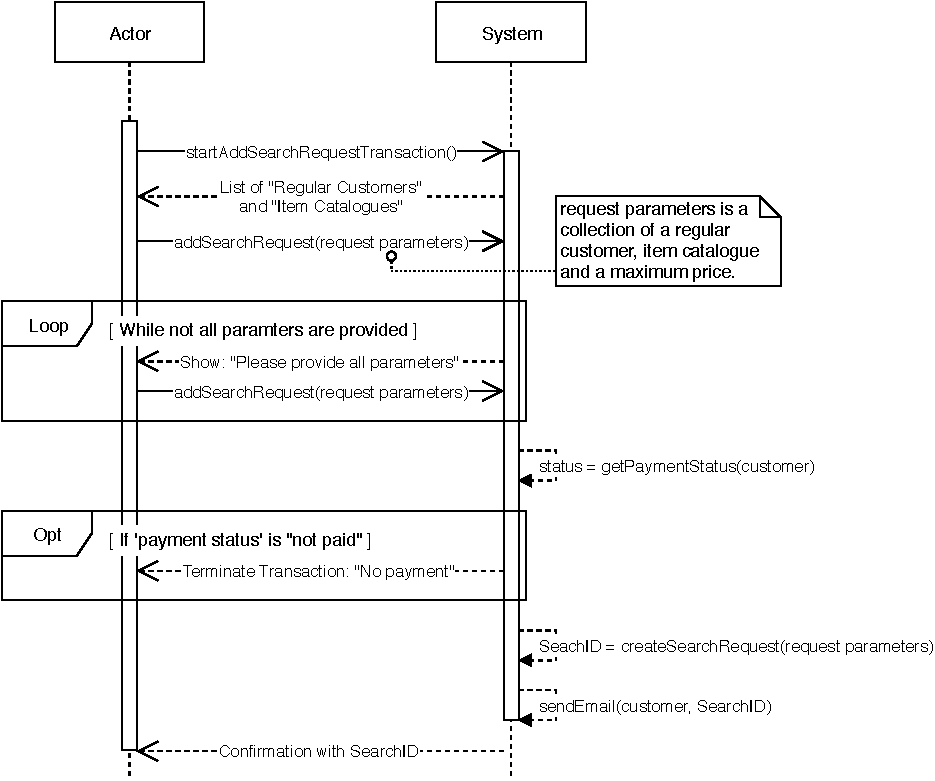
\includegraphics[scale=1]{uml/SD-bb-createsearch.pdf}
	\caption*{Interactions displayed in a System Sequence Diagram defined by the MSS and its extensions in blackbox format}
\end{figure}
\textsl{Glossary}
\begin{center}\begin{tabular}{l|l}
\textbf{Function}&\textbf{Clarification}\\\hline\hline
startAddSearchRequestTransaction()&\begin{tabular}[t]{@{}l}Starts the `add search request' transaction with the system.\end{tabular}\\\hline
addSearchRequest(request parameters)&\begin{tabular}[t]{@{}l}Requests the system to add a search request, to be created\\from the provided parameters. This request will \underline{not} register\\the search request, only ask the system to create and add\\the search request. Therefore, if not all parameters\\are provided, the request can return a failure, leaving the\\system state unchanged.\end{tabular}\\\hline
getPaymentStatus(customer)&\begin{tabular}[t]{@{}l}Gets the payment status of the customer who wants to register\\a search request. Result can be ``Paid'' or ``Not Paid''.\end{tabular}\\\hline
createSearchRequest(request parameters)&\begin{tabular}[t]{@{}l}Creates a search request from provided parameters and\\registers it to the search system. Returns the id of the new\\search request.\end{tabular}\\\hline
sendEmail(customer, SearchID)&\begin{tabular}[t]{@{}l}Sends an email to the customer, whose email address is\\known since they are a regular customer (see Domain Model).\end{tabular}
\end{tabular}\end{center}